\section{Facture d'électricité}

Sur la facture ci-dessous, certaines valeurs sont manquantes.

\begin{center}
	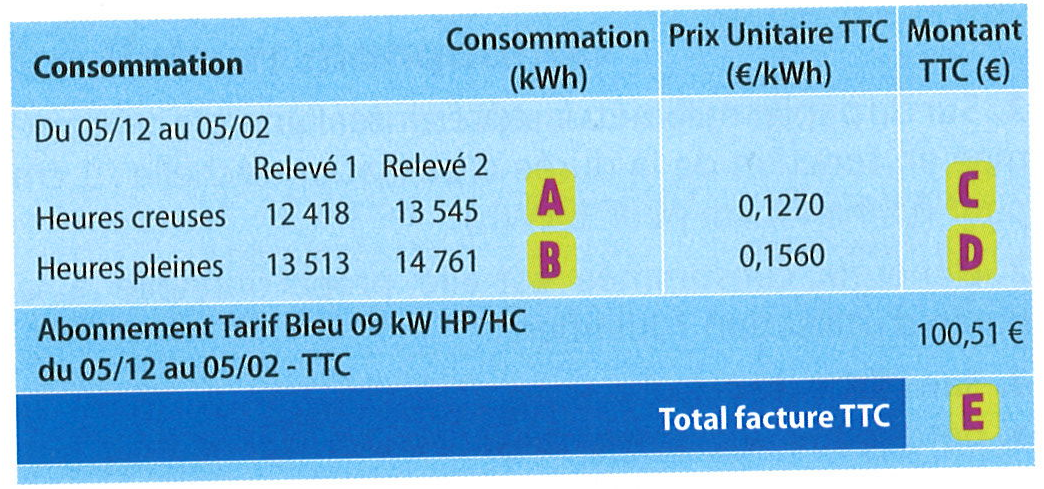
\includegraphics[scale=0.5]{img/facture}
\end{center}

\begin{questions}
	\question Retrouver par le calcul les valeurs manquantes \textbf{A} et \textbf{B}. En déduire les valeurs \textbf{C}, \textbf{D} et \textbf{E}.
	
	\fillwithdottedlines{4cm}
	
	\question Au lieu d'un abonnement <<heures creuses / heures pleines>>, on propose à un client un abonnement de \num{96.50} € avec un prix fixe pour le kWh de \num{0.1449} €. Est-ce plus intéressant ?
	
	\fillwithdottedlines{4cm}
	
	
\end{questions}